\section{Results}
\label{section:results}

The results section discusses the empirical analysis of the clustering methods tested during the implementation of the Ownership Assignment process. 
The expeirment design is simple, and designed to provide an upper-bound for performance on an optimal dataset with no noise (the Swan Valley wineries dataset.) 
The Swan Valley Wineries dataset consists of 31 wineries retrieved from OSM and \~150 objects hand-labelled across 6 of those 31 locations with ground-truth location labels. 
The objective of the experiment was to see which clustering method most accurately predicts the locaiton that the objects 'belong' to. Here accuracy is measured in two dimensions. 
First: the predicted location / true location label match. Second, the creation of the correct number of clusters (6).
K-Means and DBSCAN were tested in turn, under optimal, realistic and worst-case parameter conditions. For both DBScan and K-Means the location inference is inferred to be the location corrdinate closest to the cluster centroid. 

\subsection{K-Means}
K-Means clustering accepts the input of a collection of object coordinates, and a parameter $K$ of the number of clusters to create. 
Optimal conditions assume that the number of clusters is known ($K=6$). 
Realistic conditions assume the number of clusters is equal to the number of locations ($K=31$) and worst case conditions assume that there is only a single cluster ($K=1$). 

\begin{figure*}[h]
\centering

\begin{subfigure}[t]{.3\textwidth}
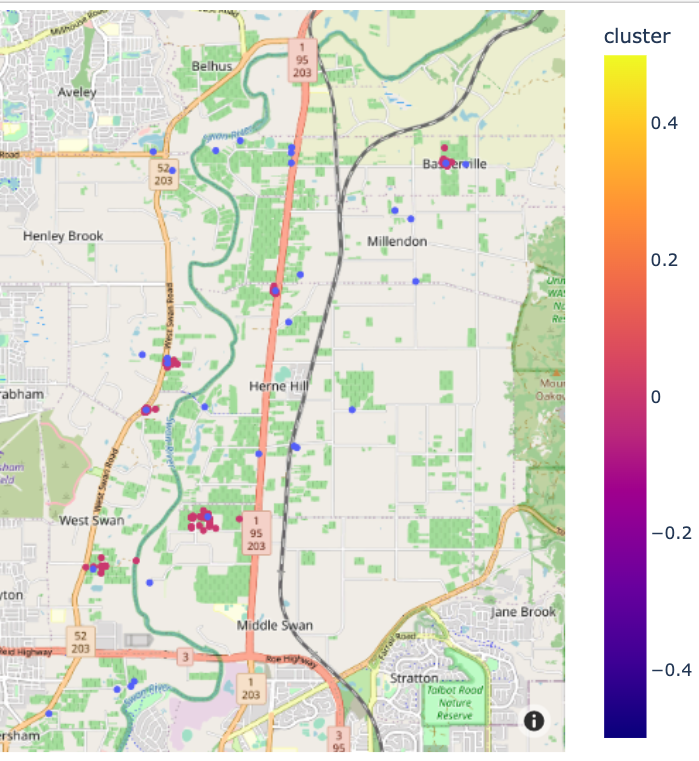
\includegraphics[width=\textwidth]{gestalt_kmeans_k1.png}
\caption{In the worst case of $K=1$ all objects are incorrectly assigned to the central location of the region.} % 
\label{fig:kmeans_worst}
\end{subfigure}
\hfill
\begin{subfigure}[t]{.3\textwidth}
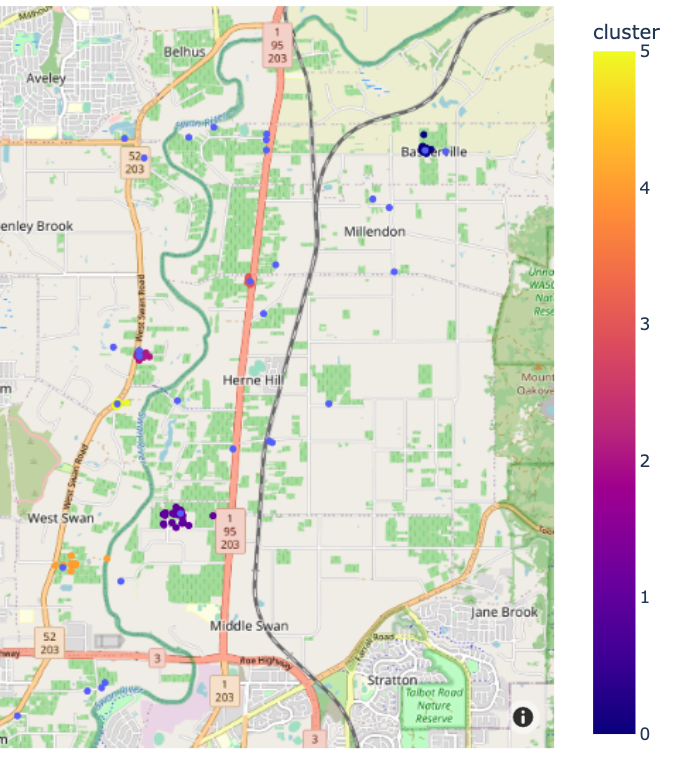
\includegraphics[width=\textwidth]{gestalt_kmeans_k6.png}
\caption{\small With optimal conditions $K=6$ the clustering performs ideally, while locations are sparse across the region.}
\label{fig:kmeans_optimal}
\end{subfigure}
\hfill
\begin{subfigure}[t]{.3\textwidth}
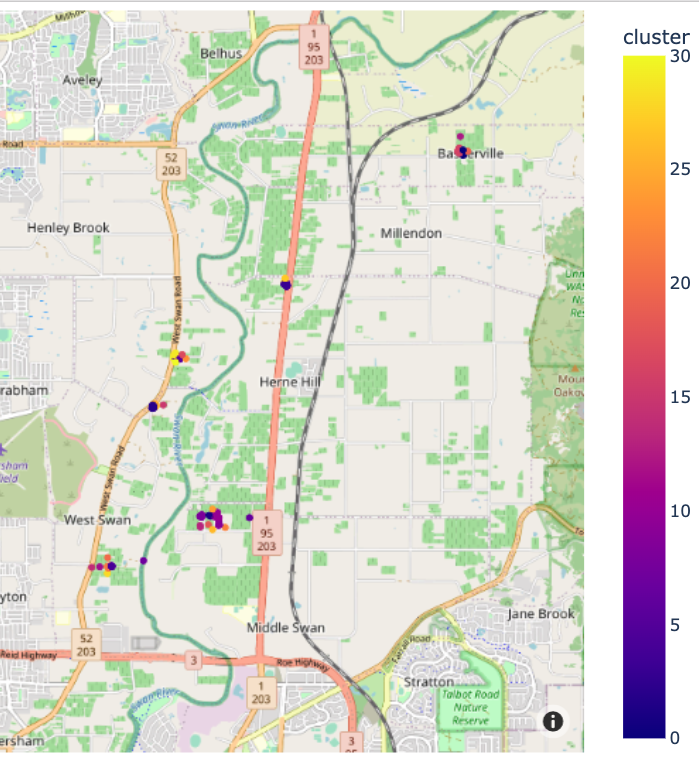
\includegraphics[width=\textwidth]{gestalt_kmeans_k31.png}
\caption{\small In realisitic settings where $K=Number of Locations$ it clusters incorrectly but assigns the correct owners. This is unlikely to hold when location density increases}
\label{fig:kmeans_realistic}
\hfill
\end{subfigure}

\caption{\textbf{K-Means Performance.} In regions with sparse location K-Means performs well even if too many clusters are created, this is not expected to hold in dense regions.}

\label{fig:kmeans_experiments}
\end{figure*}

Unsurprisingly, the optimal situation performed best with all objects assigned to their correct clusters, and all clusters assigned to their correct label. There is one reported mis-classification which was determiend to be a labelling error in the training data. Surprisingly, under 'realistic' conditions, though the number of clusters is far more than there should be, it correctly assigns the ownership of almost all objects with only 5 incorrectly labeled. Under the worst case conditions it only creates a single cluster and assigns all objects to the (same) incorrect loction. 

\subsection{DBSCAN}
The DBSCAN algorithm was introduced in 1996 by Ester et. al \cite{Ester1996}. It is a clustering algorithm that accepts the input of a collection of object coordinates, and two parameters $\epsilon$, the distance permitted between coordinates before they are considered to be in a different cluster and $N$ the number of coordinates required to be within $\epsilon$ of each other to form a cluster. 
A 2017 paper by Schubert et. al\cite{Schubert2017} provides useful guidance on turning these parameters and their experiments reveal that te value of $\epsilon$ is much more sensitive than the value of $N$. Based on their guidance, optimal conditions would see $\epsilon \leftarrow (2xdim)-1 = 3metres$. Their guidance further notes that domain knowledge should be used where appropriate so here we set ($\epsilon = 10 metres$). Realistic sets ($\epsilon = 100 metres$) and worst case sets ($\epsilon = 1000 metres$). $N=3$ in all tests. 

\begin{figure*}[h]
\centering

\begin{subfigure}[t]{.3\textwidth}
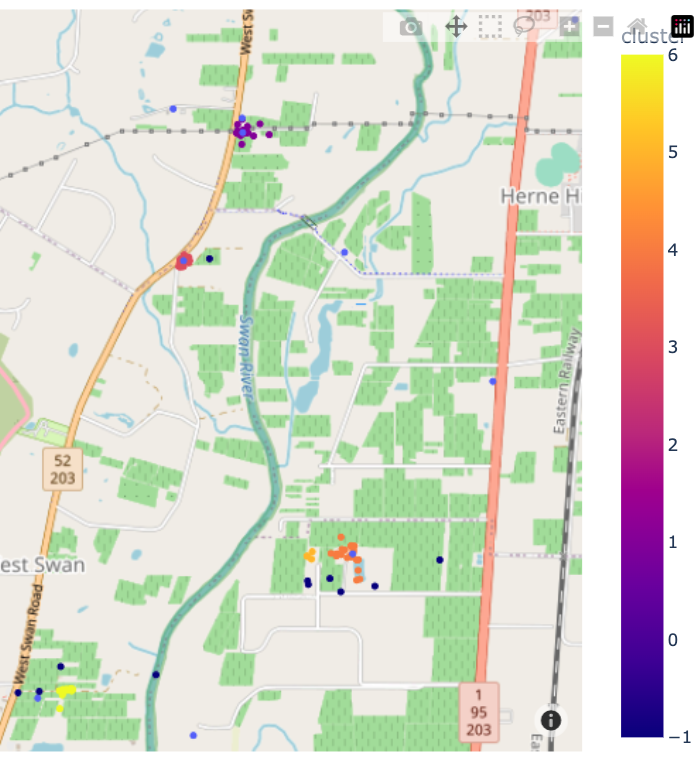
\includegraphics[width=\textwidth]{gestalt_dbscan_e10.png}
\caption{In the optimal case of $\epsilon=10$ 12 objects are incorrectly pruned as 'noise' (cluster = -1).} % 
\label{fig:dbscan_optimal}
\end{subfigure}
\hfill
\begin{subfigure}[t]{.3\textwidth}
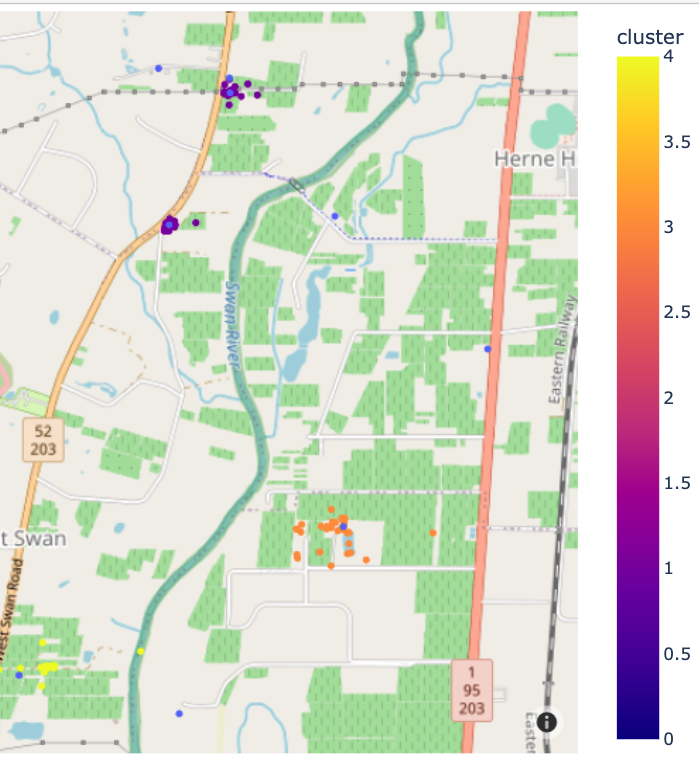
\includegraphics[width=\textwidth]{gestalt_dbscan_e100.png}
\caption{\small With realistic conditions $\epsilon=100$ the \textit{ugly duckling wines} and \textit{Little River Winery} merge because the locations are too close.}
\label{fig:dbscan_realistic}
\end{subfigure}
\hfill
\begin{subfigure}[t]{.3\textwidth}
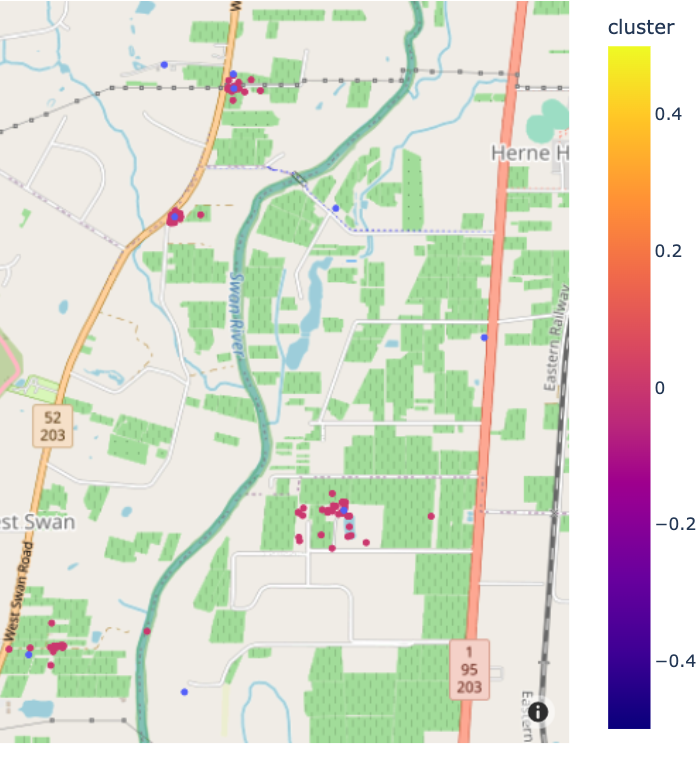
\includegraphics[width=\textwidth]{gestalt_dbscan_e1000.png}
\caption{\small In worst-case settings where $\epsilon=1000$ (too large) it groups all objects into a single cluster and incorrectly assigns to the central location of the region}
\label{fig:kmeans_worst}
\hfill
\end{subfigure}

\caption{\textbf{DBSCAN Performance.} DBSCAN performs suboptimally when locations are close togther, and when $\epsilon$ is too small or too large}

\label{fig:dbscan_experiments}
\end{figure*}

The experiments indicate that the when $\epsilon$ values are small, more of the data is regarded as 'noise' and disregarded by the clustering algorithm. With $\epsilon=10m$ it forms 6 clusters, splitting \textit{Oakover Grounds} in half, and discarding 12 objects of the ~150 as noise. Discarding objects is problematic as it degrades the recall of objects that are distant from other objects. Conversely, as $\epsilon$ increases, clusters rapidly begin to merge together. This is evident in the Winery Dataset when \textit{Ugly Duckling Wines} and \textit{Little River Winery and Cafe} are merged together, despite being clearly distict locations. The worst case, where $\epsilon$ is set too large is the merging of all objects into a single, average location, with the worst case performance of DBSCAN matching the worst case performance of K-Means with all objects being assigned to the \textit{Sitealla} winery. 

\begin{table}[h!]
	\begin{center}
		\begin{tabular}{ |c|c|c|c|c| } 
			\hline
			Algorithm & Variant & Num Clusters & Accuracy \\
			\hline
			\multirow{3}{4em}{K-Means} & $K=1$ & 1 & 0/146 \\ 
			& $K=6$ & 6 & 146/146 \\ 
			& $K=31$ & 31 & 141/146 \\ 
			\hline
			\multirow{3}{4em}{DBSCAN} & $\epsilon=10m$, $N=3$ & 7 (+ 12 'noise') & 134/146 \\ 
			& $\epsilon=100m$, $N=3$ & 7 (+ 0 'noise') & 126/146 \\ 
			& $\epsilon=1000m$, $N=3$ & 1 (+ 0 'noise') & 0/146 \\ 
			\hline
		\end{tabular}
		\label{table:clustering}
		\caption{K-Means with perfect information performs best. DBSCAN handles dense inter-location clusters and variance in intra-object cluster density poorly}
	\end{center}
\end{table}

\subsection{Error Analysis}
Examination of the errors reveal the following insights about each of the clustering techniques. 

\textbf{When K-Means clusters incorrectly, labels are still correct.} When $K$ is set to a number greater than the actual number of clusters, it fragments the true clusters. 
However, in ideal conditions like the Wineries Dataset where locations are clearly seperated, the centroids of these cluster fragments is still closest to the correct location. 
As a consequence, they are correctly labelled despite being incorrectly clustered. We expect that the accuracy will drop considerably when locations are more densely packed. However, in situations where we are aiming to process all objects and locations in a region concurrently, the number of clusters is likely to approach the number of regions. 

\textbf{DBSCAN excludes outlying examples.} To prevent all locations in a region being merged together, a small $\epsilon$ is better. However, a small epsilon increases the number of points determined to be 'noise' and hence are not added to any cluster, or provided with a label. 
The failure of DBSCAN to achieve 100\% recall of objects is problematic, as the number of objects associated with clusters should be maximised. Making $\epsilon$ larger however results in locations merging. As discussed in section \ref{section:implementation} the DVBSCAN algorithm is a promising approach that will improve the ability to use a larger $\epsilon$ to improve recall without merging adjacent clusters. 

\subsection{Summary of Experimental Results}. 
The experiments reveal that small changes in the parameters of both K-Means and DBSCAN dramatically impact the output. K-Means performed the best under optimal conditions, and better than DBSCAN under 'realistic' conditions. 
However, in datasets where locations are more densely packed, the benefit is expected to level and so experimentation with an algorithm that is able to accept as a parameter the list of locations to use as clustering centroids seeks to overcome this issue in dense localities. 
DVBSCAN is the most promising avenue for impelemting the improved ownership assignment. 
